\documentclass{article}
\usepackage{amsmath,amssymb}
\usepackage[utf8]{inputenc}
\usepackage{fullpage}
\usepackage{tej}
\usepackage{titlesec}
\titleformat{\subsection}[runin]{}{}{}{}[]

\title{Computational Physics Homework 2}
\author{Michael Albergo}
\date{11 October 2019}

\begin{document}

\maketitle

\section{Problem 1}
Problem 6.11 from the Newman textbook. This problem wants us to study the rate of convergence for the over-relaxation method (much akin to the derivation of the relaxation method in the book). 

\subsection*{a)}
We know from the book the \begin{align}
    x' = (1 + \omega)f(x) - \omega x \quad 
\end{align}
Following the convention from the relaxation method derivation, we say that the error on the solution $x^*$ for estimate $x$ is $\epsilon$ and the error for estimate $x'$ is $\epsilon'$. We want to solve for $\epsilon'$. \\

Solving for $f(x)$:
\begin{align}
    f(x) = \frac{x' - x}{1 +\omega}
\end{align}
we Taylor expand f(x) around the solution:
\begin{align}
    f(x) &= f(x^*) + f'(x^*)(x - x^*) \\
    &\approx x^* - \epsilon f'(x^*)
\end{align}
Plugging in and solving and multiplying by $1 + \omega$ gives:
\begin{align}
    x' - x &= \epsilon + \epsilon(\omega - (1+\omega) f'(x^*) \\
    x - x' &= -1* (\epsilon + \epsilon(\omega - (1+\omega) f'(x^*))
\end{align}
So then we can divide by $\epsilon((1+\omega)f'(x^*) - w)$ such that
\begin{align}
    \frac{x - x'}{\epsilon((1+\omega)f'(x^*) - w)} &= 1 - \frac{1}{((1+\omega)f'(x^*) -w)} \\
    \frac{x -  x'}{-x'  + x + \epsilon} &= 1 - \frac{1}{((1+\omega)f'(x^*) -w)} \\
    \frac{x -  x'}{\epsilon'} &= 1 - \frac{1}{((1+\omega)f'(x^*) -w)} \\
    \epsilon' &= \frac{x - x'}{1 - \frac{1}{((1+\omega)f'(x^*) -w)}} \\
    \epsilon' &\approx \frac{x - x'}{1 - \frac{1}{((1+\omega)f'(x) -w)}}
\end{align}
for x near $x*$, such that $f'(x) \approx f(x^*)$. 

\subsection*{b)}
Using the normal relaxation method, I see convergence to error $\leq 10^{-6}$ in around 13 steps. (See the jupyter notebook).

\subsection*{c)}
Using the over-relaxation method with $\omega = 0.7$, I see convergence to error $\leq 10^{-6}$ in around 5 steps. (See the jupyter notebook). Moving around the $\omega$ value generally changes the convergence to around 5-9 steps. This fits with the question's suggestion of improving to around at least half as many steps.

\subsection*{d})
Yes, there are circumstances where under-relaxation would be beneficial. Because the approximation accuracy (and convergence) is dependent on the derivative of the function, the step you take could continuously oscillate around the solution if the derivative is large. So when $f'(x)$ for x near $x^*$ is very large, you might want to take smaller steps so as to not continuously overshoot.

\section{Problem 2}
\begin{equation}
    I(\lambda) = \frac{2mhc^2 \lambda^{-5}}{e^{hc/\lambda k_B T} - 1}
\end{equation}

\subsection*{a)}

This question is basically asking us to find the critical points of $I(\lambda)$. This is done by taking the derivative of $I$ with respect to $\lambda$ and setting it equal to zero. Doing so should give us the equation they ask for.

\begin{align}
    \frac{\partial I}{\partial \lambda} &= \frac{2\pi m h^2 c^3 \lambda^{-7} e^{\frac{hc}{\lambda k_B T}}}{k_B T (e^{\frac{hc}{\lambda k_B T}} - 1)^2} - \frac{10 m h c^2 \lambda^{-6}}{(e^{\frac{hc}{\lambda k_B T}} - 1)} = 0 \\
     &= \frac{2\pi m h^2 c^3 \lambda^{-7}}{k_BT} e^{\frac{hc}{\lambda k_B T}} - \frac{10 m h c^2 \lambda^{-6}}{(e^{\frac{hc}{\lambda k_B T}} - 1)} = 0 \\
     &\rightarrow \frac{hc}{k_B T \lambda} - 5(1- e^{-\frac{hc}{k_B T}}) = 0 \\
     &\rightarrow 5e^{-\frac{hc}{k_B T \lambda}} + \frac{hc}{k_B T \lambda} - 5 = 0
\end{align}
If we say $x = \frac{hc}{k_B T \lambda}$, then 
\begin{align}
    5 e^{-x} + x - 5 = 0
\end{align}
as desired.
\subsection*{b)} See corresponding jupyter notebook: $b = 0.0028978$.


\subsection*{c)} See corresponding jupyter notebook: $T = \frac{b}{\lambda}$ and for $\lambda = 502 \times 10^{-9}$ meters, $T \approx 5772 $ Kelvin.

\section{Problem 3}

\subsection*{a)}
{\bf Implement multivariate gradient descent and demonstrate that it works.}
\\
\par First, here is evidence that the gradient descent algorithm implemented in the jupyter notebook functions properly.  Shown in Figure \ref{grad_test} is the convergence of the parameters $(x,y)$ for minimizing $f(x,y) = (x-2)^2 + (y-2)^2$.
\begin{figure}[t]
  \centering
    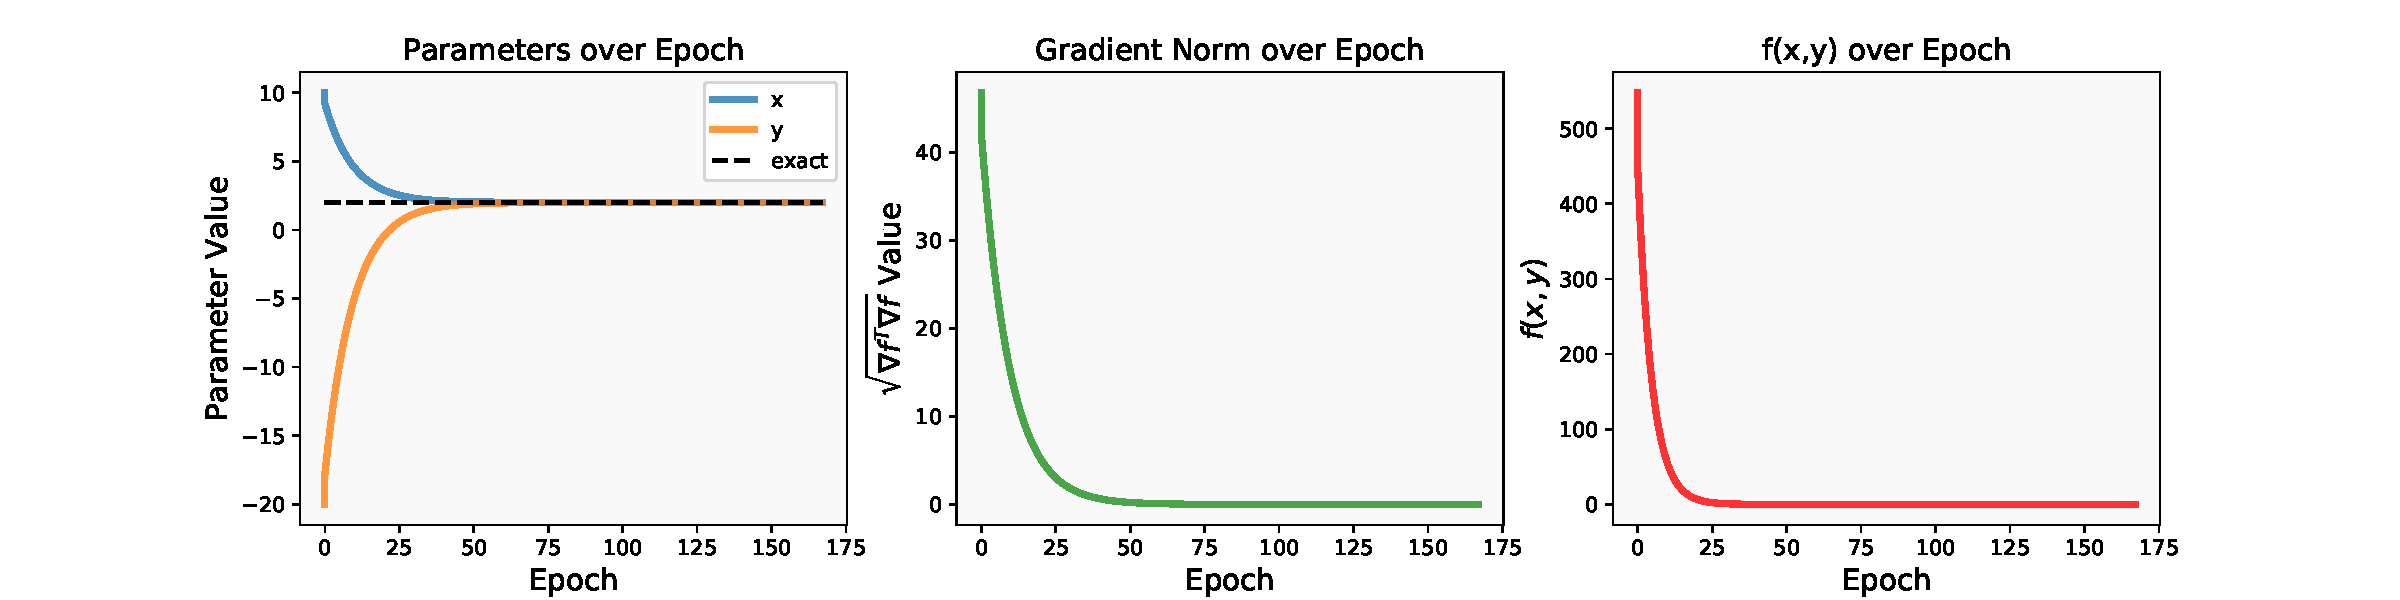
\includegraphics[width=1.0\textwidth]{gradient_test.pdf}
      \caption{Convergence of parameters while minimizing the test function $f$.}
    \label{grad_test}
\end{figure}
The implementation quickly finds the optimal parameters $(x^*, y^*)$ that minimize the function (2 and 2, respectively).


\subsection*{b)}
{\bf Show the Schechter function best fit and the chi-square convergence.}\\
\par This approach is then applied to the Schechter function data. The new goal is to minimize the $\chi^2$ of: \begin{align}
    n(M_{gal}) = \phi^* (\frac{M_{gal}}{M_{*}})^{\alpha + 1} e^{\frac{M_{gal}}{M_{*}}} \ln{10}
\end{align}
Some of the data provided was exponentiated (originally given in log base 10 form). 
\begin{figure}[h]
  \centering
    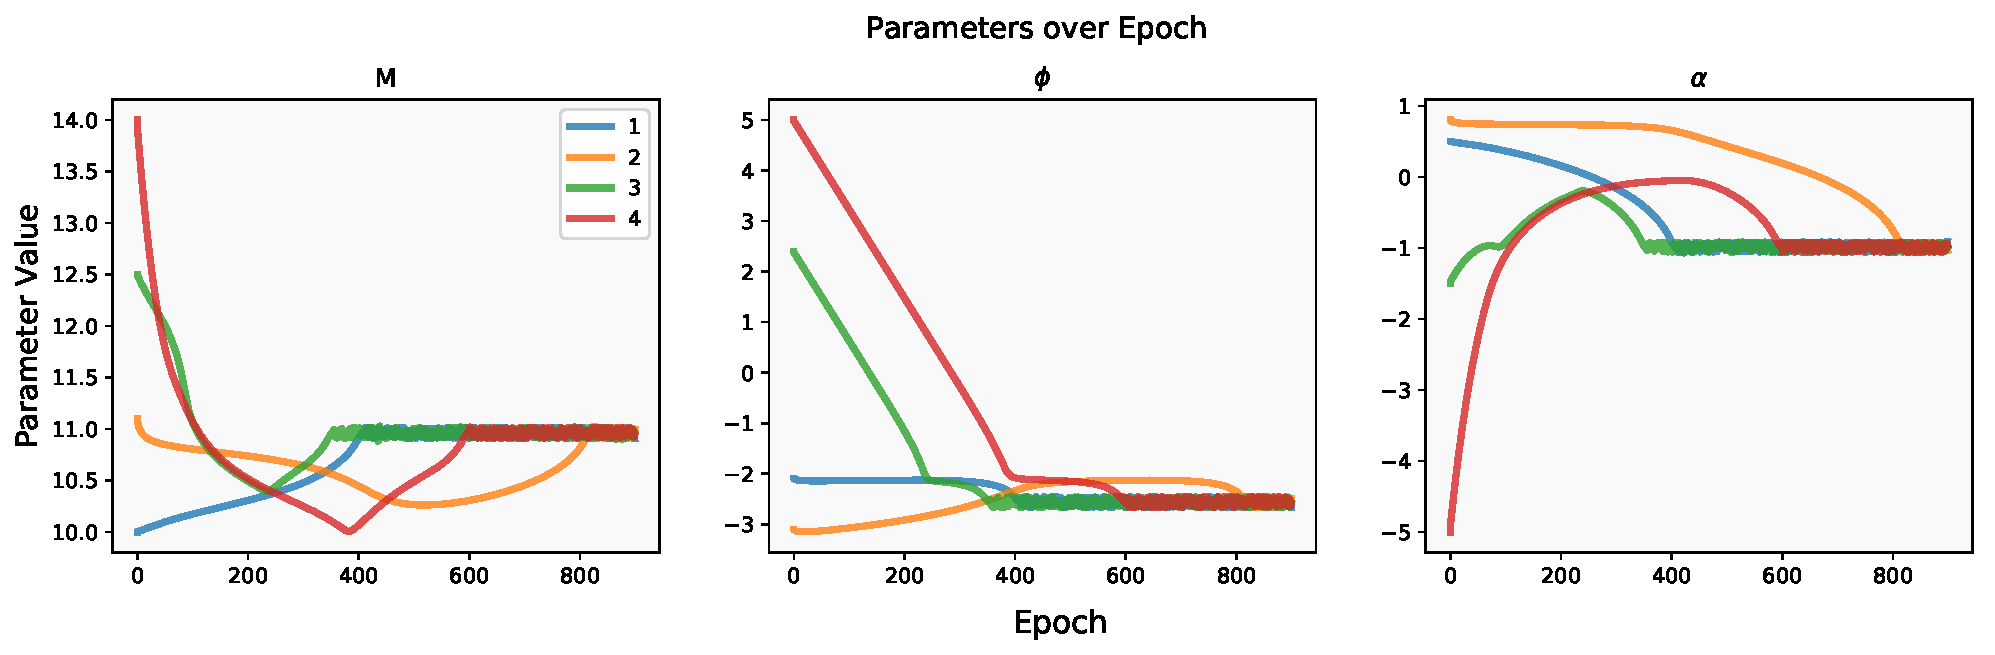
\includegraphics[width=1.0\textwidth]{param_convergenceMgal_2.pdf}
      \caption{Convergence of parameters while minimizing the test function $n(M_{gal})$.}
    \label{param_Mgal}
\end{figure}
In Figure \ref{param_Mgal} the optimal values of M, $\phi$, and $\alpha$ were found via gradient descent for 4 different trials, differing by parameter initialization. The initialization of the parameters governed the speed for which convergence was reached. These values can be found in the jupyter notebook, and were chosen to be reasonable enough that the exponents they helped define were not unstable. Plots of the log $\chi^2(n)$ over epoch are shown in Figure \ref{chi2}, for which it can be seen that the $\chi^2(n)$ value goes to and oscillates around 0. Using the converged parameters, a best fit for the Schechter was constructed for each trial. These are illustrated compared to the real data provided for the homework in Figure \ref{schechter}.

\begin{figure}[h]
  \centering
    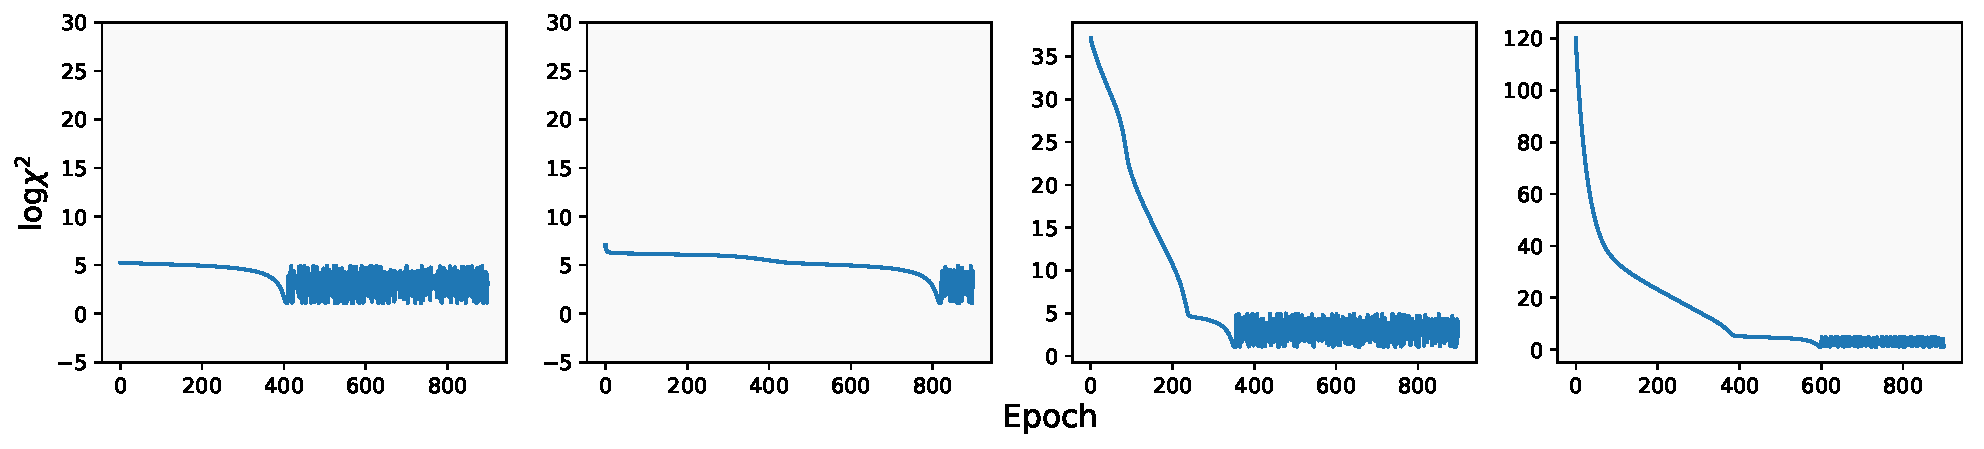
\includegraphics[width=1.0\textwidth]{chi2_2.pdf}
      \caption{Minimization of $\chi^2(n)$ for the four different trials.}
    \label{chi2}
\end{figure}

\begin{figure}[t]
  \centering
    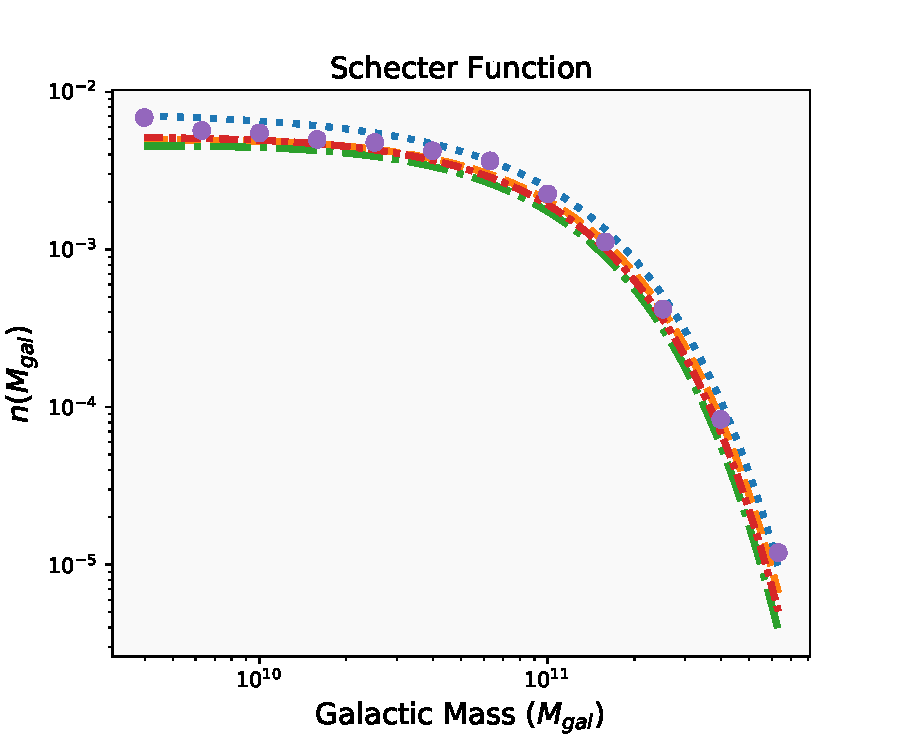
\includegraphics[width=0.6\textwidth]{schecter_function_2.pdf}
      \caption{Schechter function best fir for the four different trials. Actual data shown as purple dots.}
    \label{schechter}
\end{figure}


\end{document}
